训练集损失函数代际变化情况如下:

\begin{figure}[H]
    \centering
    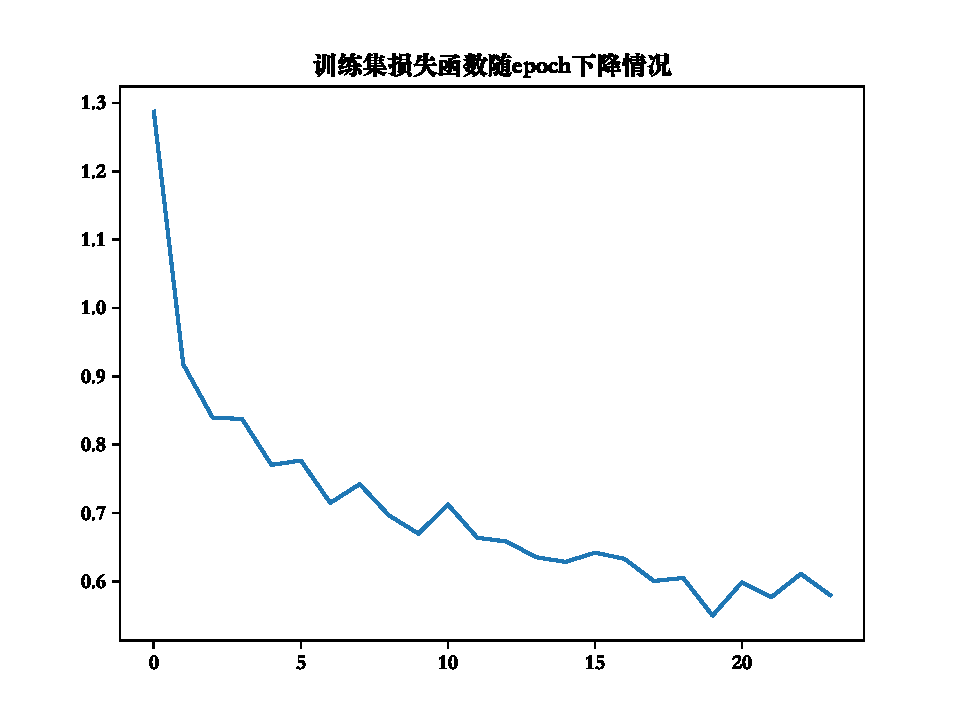
\includegraphics[width=0.6\textwidth]{figures/train-loss}
    \caption{训练集损失函数代际变化情况}
\end{figure}

可以看出损失函数大体上还是呈现一个下降的趋势, 且这个趋势会慢慢收敛, 符合预期.

测试集准确率函数代际变化情况如下:

\begin{figure}[H]
    \centering
    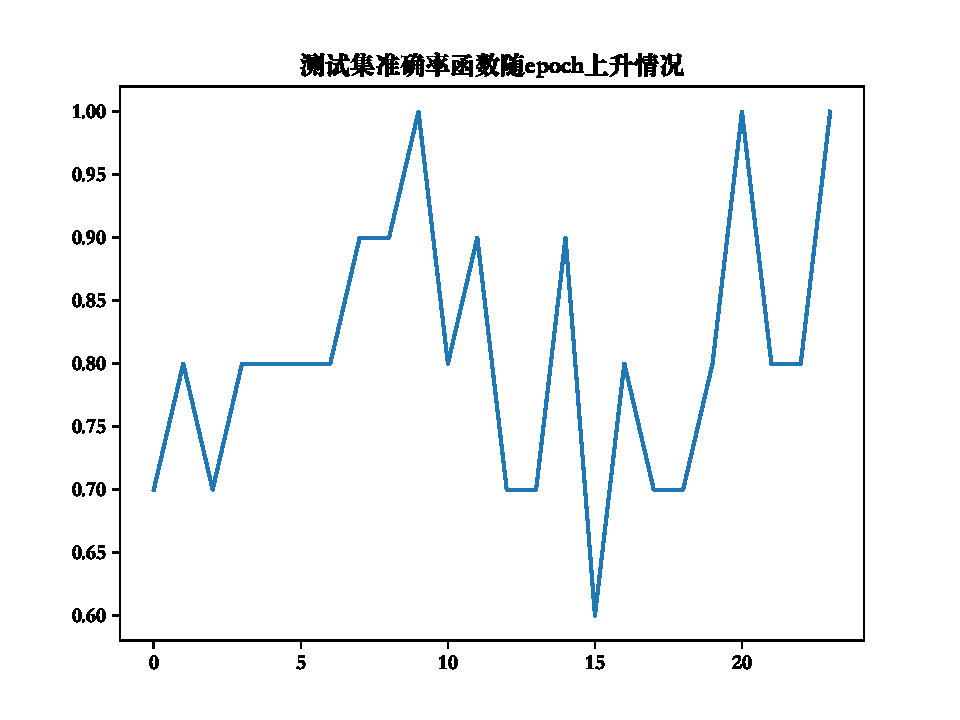
\includegraphics[width=0.6\textwidth]{figures/test-acc}
    \caption{测试集准确率函数代际变化情况}
\end{figure}

由于测试集仅有10张图片, 可以看出准确率波动性较大, 不能作为一个很好的观察结果.